% !TEX program = xelatex
\documentclass[12pt, a4paper]{article}
\usepackage[utf8]{inputenc}

\usepackage{fontspec}
\setmainfont[Ligatures=TeX]{Linux Libertine O}

\usepackage[hidelinks, colorlinks = true, linkcolor = black, urlcolor = blue]{hyperref}
\usepackage{indentfirst}
\usepackage{graphicx}
\usepackage[left=1cm,right=1cm,top=2cm,bottom=2cm]{geometry}
\usepackage{lipsum}
\usepackage{caption}
\usepackage{subcaption}
\usepackage{dirtytalk}

\title{\textbf{Ηλεκτρονική 3} \\ \textbf{Εργασία Τελεστικού Ενισχυτή}}
\author{Θεόδωρος Κατζάλης \\ ΑΕΜ:9282 \\ katzalis@auth.gr}
\date{12 Ιανουάριου 2020}


\begin{document}

\maketitle
\sloppy
\tableofcontents
\pagebreak

\section{Εισαγωγή}

Ο τελεστικός ενισχυτής που θα επιχειρήσουμε να σχεδίασουμε είναι 2 σταδιών με είσοδο ΝMOS χώρις στάδιο εξόδου και με χωρητικό φορτίο. Αξίζει βέβαια να σημειωθεί ότι συνήθως προτιμάται η χρήση PMOS εισόδου εξαιτίας επίδρασης υποστρώματος κλπ.

Ο τελεστικός είναι πάντα 2 βαθμίδων; Γιατί χρησιμοποιήσες nmos, πότε το ένα, πότε το άλλο.

Οι προδιαγραφές με βάση την εκφώνηση της άσκησης παραμετροποιημένες με το ΑΕΜ είναι οι ακόλουθες:
\subsection{Αρχικές Συνθήκες}

%\vspace{1cm}

\begin{table}[h!]
\centering
\begin{tabular}{|c|c|}
	\hline
	Προδιαγραφές & AEM=9282  \\
	\hline
	\textbf{CL} & 2.82 (pF) \\
	\hline
	\textbf{SR} &  18.82 (V/μs)\\
	\hline
	\textbf{Vdd} & 2.046 (V) \\
	\hline
	\textbf{Vss} & -2.046 (V)\\
	\hline
	\textbf{GB} & 7.82 (MHz)\\
    \hline
    \textbf{A} & 20.82 (dB)\\
    \hline
    \textbf{P} & 50.82 (mW)\\
    \hline
\end{tabular}
%\caption{}
\end{table}

\section{Περιγραφή αλγορίθμου (θεωρητική ανάλυση)}

Όσον αφορά το υπολογιστικό, θεωρητικό κομμάτι της σχεδίασης του τελεστικού ενισχυτή, ακολουθώντας τα βήματα απο τις σημειώσεις του μαθήματος, έχουμε να αναφερουμε τα εξής:

\subsection{Υπολογισμός σταθερών}

'Οσον αφορά την τάση κατωφλίου για τα MOS τραζίστορ, χρησιμοποιήσαμε τις τιμές που αναγράφονται στην περιγραφή των τρανζιστορ (KP), το οποίο θα μπορούσαμε να το υπολογίσουμε και χειροκίνητα με τον τύπο $C_{ox} = \mu_n \cdot \frac{\epsilon_{ox}}{t_{ox}}$, όπου  $\mu_n \equiv UO$ (spice model parameter). Πράγματι βλέπουμε ότι και με τους δύο τρόπους υπολογίζουμε τις ίδιες τιμές.
    
Επειδή δεν μας δίνεται κάποιο datasheet για τα συγκεκριμένα MOSFET προκειμένου να δούμε το έυρος του $V_{th}$ και τις μέγιστες και ελάχιστες τιμές, θεωρούμε ότι διατηρείται η τιμή σταθερή και ίση με αυτές που βρήκαμε απο την περιγραφή των μοντέλων. Δηλαδή $V_t(min) = V_t(max) = V_t$. Επίσης $V_{SB} = 0$ (zero body effect), οπότε $V_{to} = V_t$.

%Απο την άλλη ίσως θα μπορούσαμε να χρησιμοποιήσουμε το πινακάκι στις διαφάνεις +- 0.15

\subsection{Βήματα αλγορίθμου}    
\begin{enumerate}

    \item \textbf{Επιλογή τιμής L} (μήκος καναλιού). 
    
    Η τεχνολογία κατασκευής υποδηλώνει το ελάχιστο δυνατό μήκος καναλιού που μπορούμε να χρησιμοποποιήσουμε στην σχεδίαση μας και συνήθως επιλέγονται τιμές 1,5 ή 2 φορές αυτής της τιμής. Δεν μπορούμε βέβαια να χρησιμοποιήσουμε κάτι μικρότερο απο 0.35u. Για λόγους ευκολίας χρησιμοποιούμε την μονάδα.
    
    % Μatlab code here
    
    \item \textbf{Eπιλογή χωρητικότητας Miller}.
    
    Για να μην λειτουργεί ο ενισχυτής ως ταλαντωτής, σε συνδυασμό με την απόκλιση που μπορεί να έχει το κέρδος (βλέποντας την απόκριση συχνότητας), επίλεγεται phase margin 60 μοιρών, το οποίο απαιτεί να ικανοποιούνται οι εξής δύο συνθήκες: 
    \begin{itemize}
        \item $C_c > 0.22C_L$
        \item $g_{m6} > 10g_{m1}$
    \end{itemize}
    
    %Επιλέγουμε $C_c = 0.6204$ και δεν στρογγυλοποιούμε την τιμή, διότι αλλιώς δεν ικανοποιείται η δεύτερη συνθήκη, για την οποία θα γίνει λόγος στην συνέχεια.
    
    Επιλέγουμε $C_c = 0.6204\approx1$. 'Επειτα την στρογγυλοποίηση, όπως θα δούμε και στην συνέχεια, η δεύτερη συνθήκη δεν ισχύει για την δεδομένη τιμή $g_{m1}$, οπότε τελικά θα θεωρήσουμε $g_{m6} = 10g_{m1}$.
    
    \item Ρεύμα πόλωσης $Iref = I5 = I8$ ($I_7 \neq I_{ref}$, εξαιτίας συνθήκης για DC offset)
    
    \item Εύρεση $S_3 = (W/L)_3$. Βρίσκουμε $\leq1$, οπότε $S_3 = 1$.
    
    \item Έλεγχος $p_3 > 10 GB$.
    
    \item
\end{enumerate}

\subsection{Τελικές τιμές}

Πινακάκι για ρεύματα και W.

\section{Προσομοίωση SPICE}

Χρησιμοποιήσαμε για NMOS και PMOS τα μοντέλα mbreakN3 και mbreakP3 αντίστοιχα ($V_{SB} = 0$) και θέσαμε τις απαιτούμενες τιμές του κυκλώματος με αυτές του αλγρορίθμου. Μια πρώτη παρατήρηση σχετικά με τα ρεύματα είναι ότι $I_1 = I_2 = I_3 = I_4 = 10.19 \approx I_{ref}/2 = 9.94u$, η τιμής του αλγορίθμου. Βέβαια έχουμε μεγάλη απόκλιση για τα $I_6 = I_7 \approx 300u$, $50\%$ αύξηση. Θεωρούμε ότι ο αλγόριθμος μας είναι σωστός και συνεχίζουμε να δούμε αν καλύπτονται οι προδιαγραφές ή κατα πόσο αποκλίνουν.

\begin{figure}[h!]
	\centering
	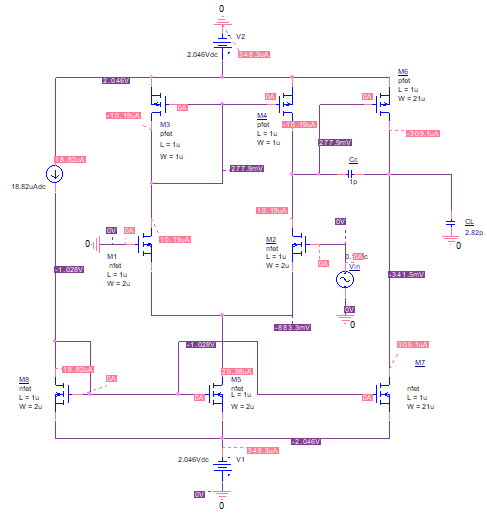
\includegraphics[width = \textwidth, height = .4\textheight, keepaspectratio]{assets/base.png}
	\caption{Κύκλωμα προσομοίωσης τελεστικού ενισχυτή}
\end{figure}

\subsection{Έλεγχος προδιαγραφών}

Για τις ακόλουθες δύο προδιαγραφές κάνουμε AC sweep και προσθέτουμε τα κατάλληλα traces.

\subsubsection{A και GB}

\begin{figure}[h!]
	\centering
	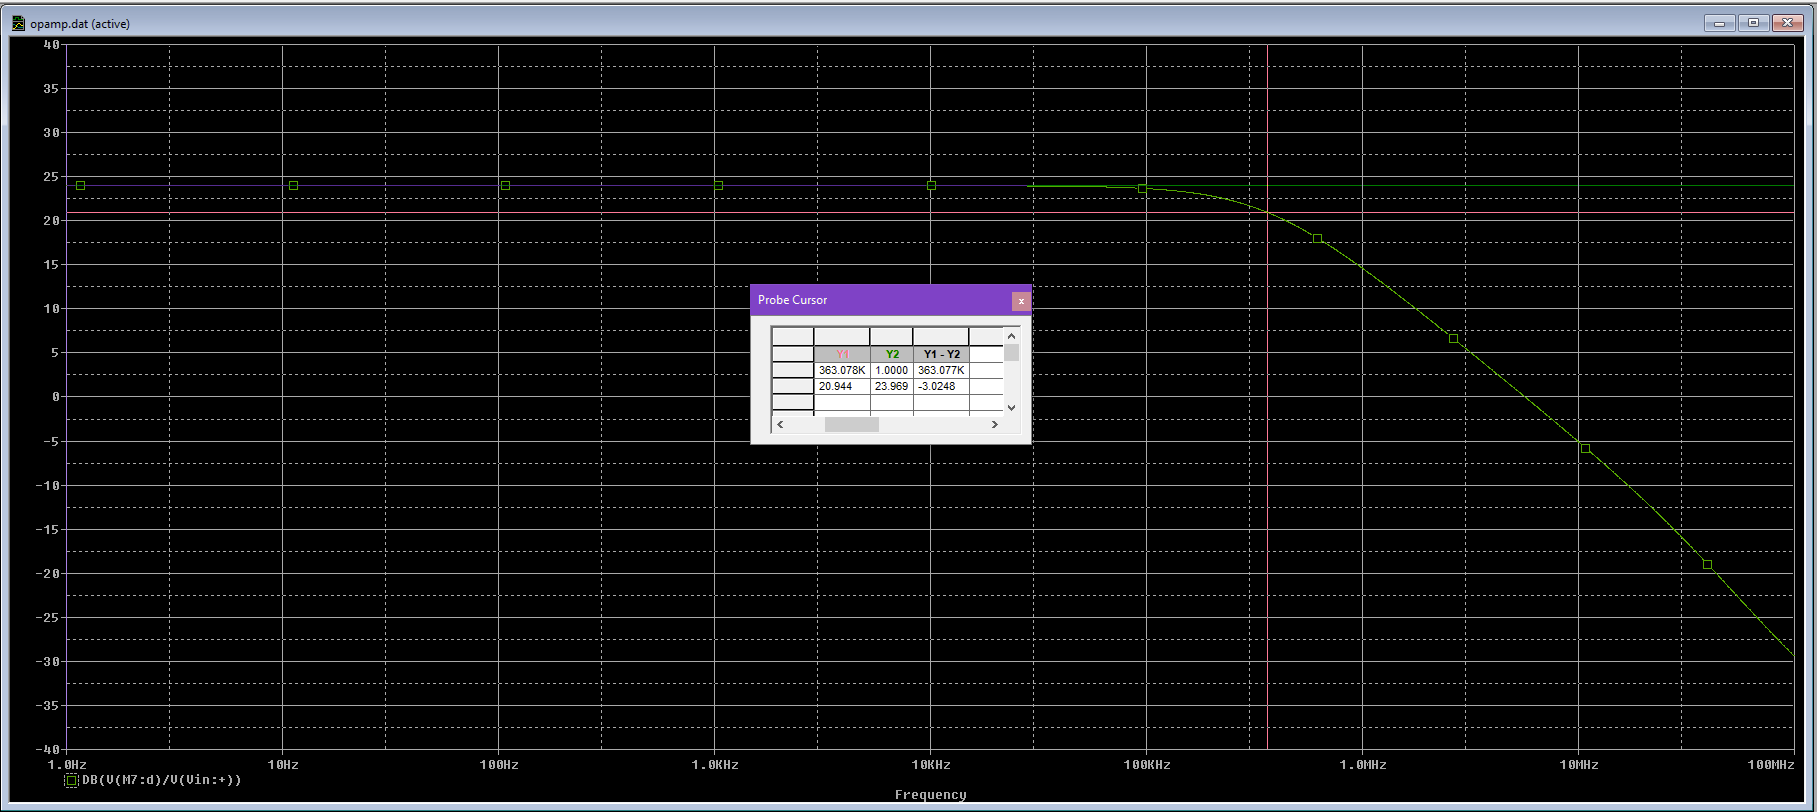
\includegraphics[width = \textwidth, height = .25\textheight, keepaspectratio]{assets/gain_GB.png}
	%\caption{Κύκλωμα προσομοίωσης τελεστικού ενισχυτή}
\end{figure}

Βλέπουμε ότι έχουμε total dc gain ίσο με 24dB (327.21), το οποίο αποκίνει απο την θεωρητική τιμή (50dB), ωστόσο είναι πάνω απο την προδιαγραφή των 20.82dB.

Για να υπολογίσουμε το GB, βρίσκουμε την συχνότητα για την οποία το κέρδος έχει μειωθεί κατα 3dB. 'Οπως φαίνεται και απο το Probe Cursor, η τιμή της συχνότητας που αντιστοιχεί στα 21 dB είναι 363ΚHz. Συνεπώς:

\[  GB = \abs{A} \cdot f_H = 326.21 \cdot 363KHz \approx 118 > 7.82 MHz \]

Πληρείται δηλαδή και η προδιαγραφή για το Gain Bandwidth.

\subsubsection{Περιθώριο φάσης}

\begin{figure}[h!]
	\centering
	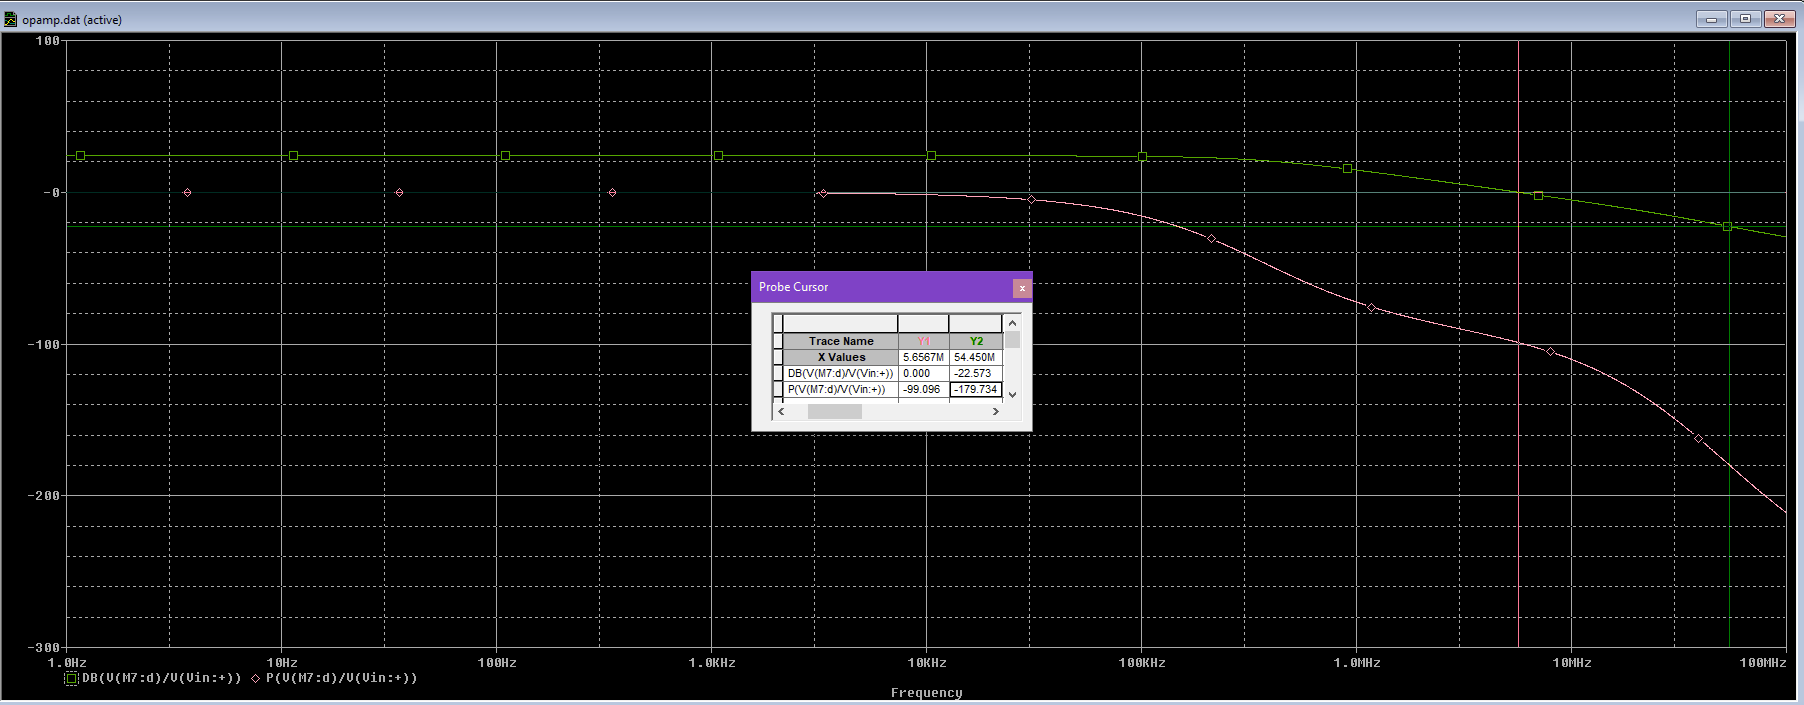
\includegraphics[width = \textwidth, height = .25\textheight, keepaspectratio]{assets/phase_margin.png}
	%\caption{Κύκλωμα προσομοίωσης τελεστικού ενισχυτή}
\end{figure}

Βλέπουμε ότι για 0 dB κέρδους, η τιμή της φάσης αντιστοιχεί σε $-99^o$. Οπότε έχουμε περιθώριο φάσης $180 - 99 = 91^ο$. Θα προσπαθήσουμε στη συνέχεια να το φτάσουμε κοντά στο 60. 

\subsubsection{Slew rate}

Μετατρέπουμε την συνδεσμολογία σε συνδεσμολογία μοναδιαίου κέρδους βραχυκυκλώνοντας την αναστρέφουσα είσοδο με την έξοδο. Αλλάζουμε και την πηγή και έχουμε ως είσοδο τετραγωνικούς παλμούς διάρκειας δες τοπικ 2018 και 2017 για τους χρόνους και τα σχετικά.



\begin{figure}[h!]
     \begin{subfigure}[b]{0.5\textwidth}
         \centering
         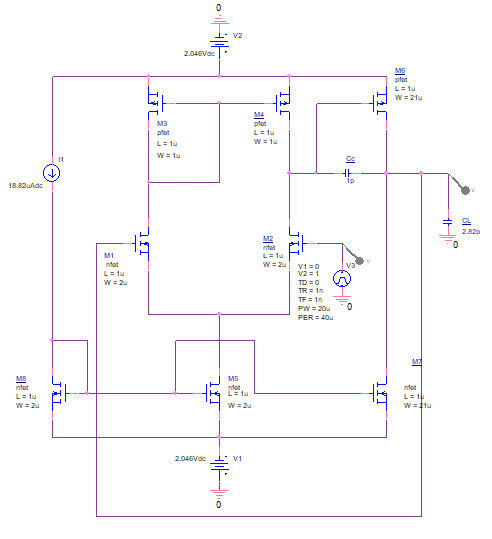
\includegraphics[height=.4\textheight, width=\textwidth, keepaspectratio]{assets/slew_rate_circuit.png}
    \caption{V3 binary search}
     \end{subfigure}
     \begin{subfigure}[b]{0.5\textwidth}
         \centering
         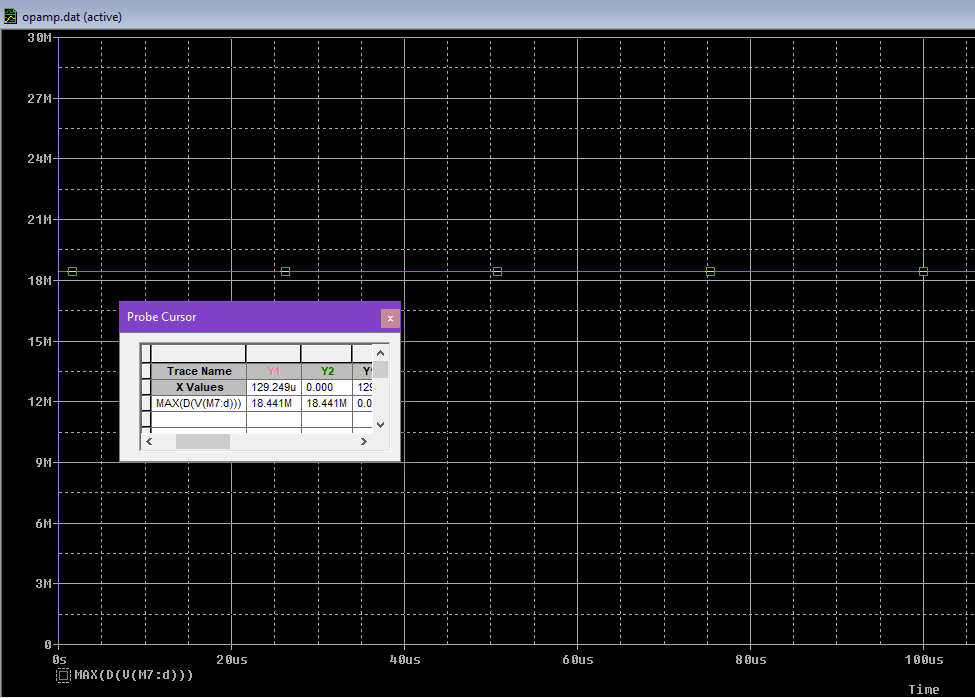
\includegraphics[height=.4\textheight, width=\textwidth, keepaspectratio]{assets/slew_rate.png}
         \caption{V4 linear search} 
     \end{subfigure}
\end{figure}

Βρίσκουμε $18.441  \approx 18.82 MV/sec (V/μs)$. Δηλαδή για πολύ λίγο δεν πιάνουμε την προδιαγραφή.

\section{Tuning}

Όπως είδαμε προηφουμένως, οι τιμές για το περιθώριο φάσης και του ρυθμού ανόδου (slew rate) δεν ικανοποιούν τις προδιαγραφές. Παράλληλα θα προσπαθήσουμε να ενισχύσουμε και το κέρδος τάσης. Με βάση το ακόλουθο πινακάκι και παραμετρικές αναλύσεις καταλήξαμε στα εξής:

\begin{figure}[h!]
	\centering
	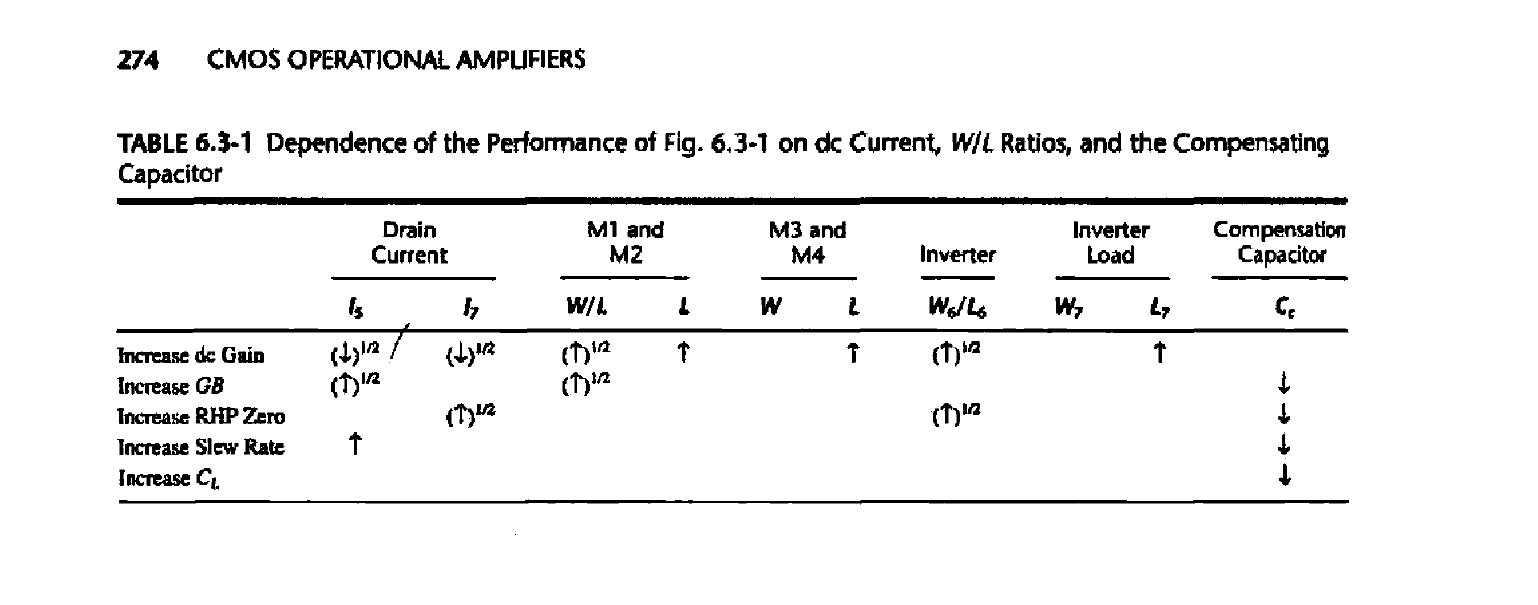
\includegraphics[width = \textwidth, height = .2\textheight, keepaspectratio]{assets/tuning_table.png}
	%\caption{Κύκλωμα προσομοίωσης τελεστικού ενισχυτή}
\end{figure}

\subsection{Α και GB}

\subsection{Phase margin}

\subsection{Slew rate}


%Μάλλον το ΑΕΜ και  η προσεκτική γραφή του αλγορίθμου, συνυπολογίζοντας συνθήκες όπως $g_{m6} \geq 10 \cdot g_{m1}$ και στρογγυλοποιώντας τους λόγους, οδηγηθήκαμε στο να μην χρειάζεται να κάνουμε tuning. Ωστόσο αξίζει να σημειωθεί ότι υπάρχει ένα πολύ βοηθητικό πινακάκι το οποίο ενδεχομένως θα μπορούσαμε να το χρησιμοποιήσουμε για να μεταβάλλουμε τις τιμές. Ενδεικτικά θα προσπαθήσουμε για παράδειγμα να αυξηθεί το κέρδος. 

%Φυσικά στο tuning θα πρέπει να μεταβάλουμε τα W με προσεκτικό τρόπο και να μην ξεχνάμε ότι υπάρχουν καθρέπτες ρεύματος για τους οποίους οι λόγοι θα πρέπει να είναι ταιριασμένοι.

\section{Παραμετρική ανάλυση θερμοκρασίας}

Απο 0-70.

\subsection{Πηγή widlar}

\end{document}
